\subsection{Introduction}
\label{subsec:introduction2}
A TPU is similar in nature to a GPU or even that of a CPU: they are the ones who are performing the computations within a system.
What distinguish the TPU from the rest is how and what kind of computations are being carried out.
While GPUs and CPUs are considered general purpose, TPUs are an application-specific integrated circuit (ASIC)~\cite{b6}.
Developed by Google, they are built to accelerate performance of Machine Learning (ML) related applications, particularly their linear algebraic processes that involve matrices.
This is also reflected by the hardware incorporated into them.
As a consequence, however, they cannot do much else, at least not efficiently.
The Tensor Processing Unit (TPU) has currently evolved to its fifth version.
However, for the purposes of this work, only TPUv4 will be discussed, highlighting its important features.

\subsection{Structure}
\label{subsec:structure}
There are 2 main components to a TPU chip: High Bandwidth Memory (HBM) and the Tensor Cores (TC).
The HBM is an on-chip memory allowing for larger models and bigger batch sizes to utilize.
The TCs on the other hand consist of many multiply-accumulators; the special hardware that allows for an increase in speed for the matrix-related operations.
These multiply-accumulators are all arranged in an array-like structure, called the systolic array structure, within the chip.

Google’s TPU machine consists of thousands of these TPU chips (as of TPUv4, there are 4096 chips placed inside).
Within the machine itself, the chips are arranged physically as separate 4 x 4 x 4 cube but the inner networking between the chips, their logical connection, is more flexible and can be defined by the user.
For instance, by default, the connections would resemble a torus.
Furthermore, within this system, a CPU is also in use.
With TPUv4, there is one CPU for every 4 TPU chips resulting in around 1000 CPUs in total.

The TPU works by first loading parameters from the HBM into individual multiply-accumulators and then feed the data/input/activation to one row/column of the array-like architecture.
The results of one computation feed the next one, and so on, similar to how a ripple-carry adder works.

\subsection{TPUv4}
\label{subsec:tpuv4}
The main improvements introduced by TPUv4 mainly handle around the subject of scale and reliability using Google's very own advancement in optical switches \cite{b7}.
Additionally, just as any other kind of iteration, the TPUv4 also improves certain aspects of the system.
For example, the storage of embeddings is dealt by introducing appropriate hardware architectures and a way that allows for a better compatibility between hardware and the model was also introduced.

\subsubsection{Reconfigurable Optical Switches}
The TPUv4 is equipped with 4096 TPU chips.
While this quantity might not appear significant, it becomes noteworthy when contrasted with the TPUv3, which only had 1024 chips.
The sheer size of the TPUv4 renders electrical switches useless due to ``electrical interconnect'' limitations.
To solve this, optical switches were used.
In particular, Google's Palomar Optically Configurable Switches (OCS).
They are based on Micro-Electro-Mechanical Systems that can send light both ways in a fiber by employing what is called a ``circulator''.

\begin{figure}[htbp!]
    \centerline{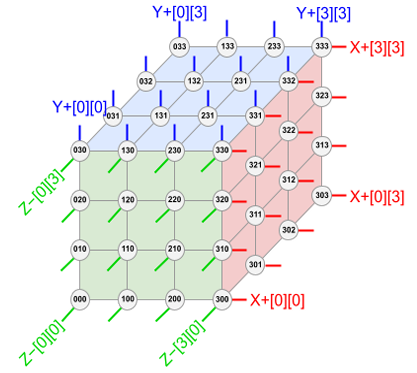
\includegraphics[width=0.2\textwidth]{images/tpu_cube}
    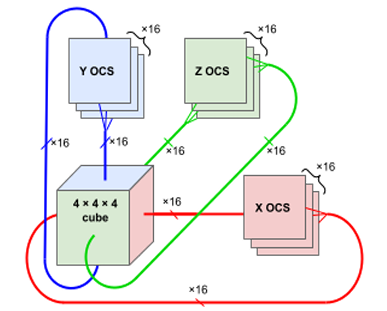
\includegraphics[width=0.2\textwidth]{images/tpu_connectivity}}
    \caption{OCS Architecture.}
    \label{fig:ocsarch}
\end{figure}

``Fig.\ref{fig:ocsarch}'' illustrates how the OCSs are connected.
This cube, a 4 x 4 x 4, is part of the TPU machine that consists of many TPU chips that must be connected to the OCS\@.
A cubic arrangement of 64 chips is considered due to nicer bisection bandwidth and for convenience in storage.
To connect, each side and its corresponding opposite side of the cube are connected to the same OCS\@.
In total, for TPUv4, there are typically 3 * 16 = 48 OCSs for a single machine.

The OCS brings a multitude of benefits.
The first being availability and deployment benefits.
Being flexible and having better performance allows TPUv4 to still provide good services, even when some chips of the system may not be available.
And because the OCSs bring some sort of independence to the system (particularly, it made each rack of the machine more independent), not all chips are needed to ensure operability.

Second, the most obvious one, configurability.
The OCS greatly simplifies scheduling and networking within the system due to its great switching speed.
For instance, it no longer has to search for many contiguous chips during scheduling as required by the previous version and the OCS. It allows modularity between users (the whole system can cater to multiple users) which enhances security.
Finally, the logical connection can be easily reconfigured to one's topological needs, typically to exploit different kind of parallelisms (i.e., Data, Model, and Pipeline parallelism), as ``rewiring'' the system mostly involves reprogramming the routes of the OCS\@.

\subsubsection{SparseCore}
Like any other computers dealing with ML, this one is for dealing with embedding.
In particular, where to store the lookup tables from the embedding process.
The main problem here is that the lookup operations will cause a bottleneck for the chips due to memory accesses, inter-chip communication, etc.
As they are more suited for dense arithmetic operation.

In this context, there were two possible solutions: either put it in the CPU or put it in the tensor cores themselves.
The CPU approach would introduce a bottleneck during the next iterations by Amdahl’s law; in comparison, there is a 4:1 TPUv4 to host CPU ratio.
On the other hand, putting it in the TC would be suboptimal due to them being optimized for dense operations.
A way out of this is to use both the HBM and the dedicated Inter-Core Interconnect (ICI) network which are embedded in the chips.
With these in mind, comes SparseCore (SC).
It is an additional hardware put in the machine for dealing with embedding training.
SC uses the HBM and a dedicated ICI network while operating in a sea of cores configuration creating a flat, globally addressable memory space.

Although SC seems to only handle storage of embeddings, it actually behaves almost as a whole package to deal with sparse data related operations.
Mainly, it consists of 16 compute tiles and 5 Cross-Channel inputs for performing preprocessing of the sparse input.
Each compute tile consists of a fetch unit, Single Instruction Multiple Data (SIMD) Vector Processing Unit, the Sparse Vector Memory for storing data read from the fetch unit, and the flush unit utilized during backward propagation.

\subsubsection{Platform-Aware Neural Architecture Search}
Platform-Aware Neural Architecture Search or PA-NAS has a goal to configure both the ML model and the TPU topology to benefit from each other as much as possible.
In particular, with the mention of SC, a model in the TPU might need to use both SC and TC efficiently.
PA-NAS optimizes operations related to this to achieve ``pareto-optimal performance and quality''.